\section{Closure properties of languages with polynomial rational indices}
\label{sec:closure}
Given a context-free language $L$ with a polynomial rational index, it is interesting to find which language operations preserve this property.  Boasson et al. \cite{RatBasic} give following useful relations for polynomial indices of two languages $L$ and $L'$.
\begin{theorem}[\cite{RatBasic}]
Context-free languages with polynomial rational indices are closed under intersection with a regular language, union, concatenation, homomorphism and inverse homomorphism. More precisely,
\begin{itemize}
\item $\rho_{L \cup L'}(n) \le  \max{(\rho_L(n), \rho_{L'}(n))} $
\item $\rho_{LL'}(n) \le \rho_L(n) + \rho_{L'}(n)$
\item $\rho_{L \cap R}(n) \le \rho_L(nm)$, where $R$ is a regular language recognised by an $m$-state automaton
\item $\rho_{h(L)}(n) \le \rho_L(n)$ and $\rho_{h^{-1}(L)}(n) < n(\rho_L(n) +1)$, where $h: \Sigma^* \rightarrow \Delta^*$ is a homomorphism.
\end{itemize}
\end{theorem}
From the relations above it is easy to see that the family of context-free languages with polynomial rational indices is a full trio. Every full trio is closed under prefix and quotient with regular languages. Obviously, CFLs with polynomial rational indices languages are closed under reversal.  Next we show that context-free languages with polynomial rational indices are closed under the Kleene star and insertion of a regular language (or context-free language with a polynomial rational index).
\begin{theorem}
Context-free languages with polynomial rational indices are closed under the Kleene star and insertion of a regular language  (or context-free language with a polynomial rational index). Particularly,
\begin{itemize}
\item $\rho_{L^{*}}(n) \le n(\rho_L(n))$
\item $\rho_{L_{INSERT(K)}}(n) \le \rho_L(n) + \rho_{K}(n)$
\end{itemize}
\end{theorem}
\begin{figure}
\centering
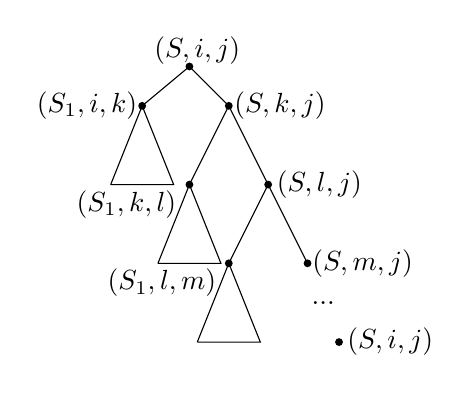
\begin{tikzpicture}
\draw(0, 2.5) -- (0.4,3.5) -- (0.8, 2.5) -- (0, 2.5) ;
\draw (0.4,3.5) -- (1,4) -- (1.5, 3.5);
\draw  (1,2.5) -- (1.5, 3.5) -- (2, 2.5);
\draw(0.6, 1.5) --  (1,2.5) --  (1.4, 1.5) -- (0.6, 1.5);
\draw(1.5, 1.5) -- (2, 2.5) -- (2.5, 1.5);
\draw (1.1, 0.5) -- (1.5, 1.5) -- (1.9, 0.5) --  (1.1, 0.5);


 
\node (q1) at  (1.1, 4.2) {$(S, i,  j)$}; 
\node (q1) at  (2.7, 1) {$...$}; 
\node (q1) at  (3.55, 0.5) {$(S, i,  j)$}; 
\node (q1) at  (2.15, 3.5) {$(S, k,  j)$}; 
\node (q1) at  (-0.3,3.5) {$(S_1, i,  k)$}; 
\node (q1) at  (2.65, 2.5) {$(S,l,j)$}; 
\node (q1) at  (0.2, 2.25) {$(S_1, k, l)$}; 
\node (q1) at  (3.2, 1.5) {$(S, m, j)$}; 
\node (q1) at  (0.65, 1.25) {$(S_1, l, m)$}; 



\node [circle, fill=black, inner sep = 1pt, minimum size=0.5pt] at (0.4,3.5) {};
\node [circle, fill=black, inner sep = 1pt, minimum size=0.5pt] at (1,4) {};
\node [circle, fill=black, inner sep = 1pt, minimum size=0.5pt] at (1.5, 3.5) {};
\node [circle, fill=black, inner sep = 1pt, minimum size=0.5pt] at  (2, 2.5) {};
\node [circle, fill=black, inner sep = 1pt, minimum size=0.5pt] at (1,2.5) {};
\node [circle, fill=black, inner sep = 1pt, minimum size=0.5pt] at (1.5, 1.5) {};
\node [circle, fill=black, inner sep = 1pt, minimum size=0.5pt] at (2.5, 1.5){};
\node [circle, fill=black, inner sep = 1pt, minimum size=0.5pt] at (2.9, 0.5){};
%\node [circle, fill=black, inner sep = 1pt, minimum size=0.5pt] at  (2.2, 1.9) {};
\end{tikzpicture}
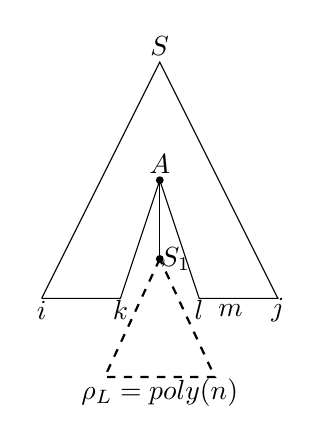
\begin{tikzpicture}
\draw(0,0) -- (1.5, 3) -- (3, 0) -- (2, 0) -- (1.5, 1.5) -- (1, 0) -- (0,0);
\draw(1.5, 1.5) -- (1.5, 0.5);
\draw [thick, dashed](1.5, 0.5) -- (0.8, -1) -- (2.2, -1) --  (1.5, 0.5) ;

\node [circle, fill=black, inner sep = 1pt, minimum size=0.5pt] at (1.5, 1.5) {};
\node [circle, fill=black, inner sep = 1pt, minimum size=0.5pt] at (1.5, 0.5) {};

\node (q1) at  (1.5, 3.2) {$S$}; 
\node (q1) at   (1.5, 1.7) {$A$}; 
\node (q1) at   (1.7, 0.5) {$S_1$}; 
\node (q1) at   (1.5, -1.2) { $\rho_{L} = poly(n)$}; 
\node (q1) at  (0,-0.15) {$i$}; 
\node (q1) at  (1,-0.15) {$k$};
\node (q1) at  (2,-0.15) {$l$};
\node (q1) at  (3,-0.15) {$j$};
\node (q1) at  (2.4,-0.15) {$m$};


\end{tikzpicture}
\\
	\caption{Parse trees after applying the Kleene star operation (left) and insersion of the language with a polynomial rational index (right).}
\label{closure}
\end{figure}
\begin{proof}
\textit{(The Kleene star)} Let $G = (\Sigma, N, P, S)$ be a grammar in Chomsky normal form and $L(G)$ be a language with polynomial rational index. Consider the language $L^{*}$. A grammar $G'$ for $L^{*}$ can be constructed from $G$ as usual by renaming start nonterminal $S$ to $S_1$ and adding a new start nonterminal $S$ with production rules $S \rightarrow S_1S$ and $S \rightarrow \varepsilon$. Consider a labeled parse tree for $G'$ and some NFA (see Figure~\ref{closure} (left)), constructed in the same way as a tree from the proof of Lemma~\ref{lem:treeheight}. Suppose that this tree is a parse tree for the shortest word $w$ in the intersection of $L(G')$ and an arbitrary $n$-state NFA with the start and final states $i$ and $j$ respectively. Such tree has no more than $n$ subtrees rooted by $S_1$, because there is no more than $n$ triples in form of $(S, x, j)$ for a fixed $j$ (otherwise $w$ is not the shortest). Every tree rooted by $S_1$ has at most polynomial number of leaves, because $L(G)$ has a polynomial rational index. Thus $\rho_{L^{*}}(n) \le n(\rho_L(n))$.
\\
\textit{(Insertion of a regular language (or context-free language with a polynomial rational index))} Proof by contradiction. Consider a parse tree $T$ for the shortest word $w$ from the intersection of $L_{INSERT(K)}$, where $K$ is a language with a polynomial rational index, and an arbitrary $n$-state NFA $\mathcal{A}$ with the start and final states $i$ and $j$ respectively (see Figure~\ref{closure} (right)). Let $w = l(i \pi j)$. Suppose that $T$ has exponential on $n$ number of leaves and, hence, a path $i \pi j$ has an exponential length. A subtree rooted by $S_1$ belongs to the grammar, which generates words from $K$, therefore this subtree has at most polynomial number of leaves by the definition of rational index. So, the whole tree, except the subtree rooted by $S_1$, has an exponential number of leaves. Suppose $m$ is the next state in the shortest path from $l$ to $j$ in $i \pi j$. Then one can construct from $\mathcal{A}$ a new $n$-state NFA $\mathcal{A'}$, where state $k$ has an edge to $m$ labeled the same way as the transition from $l$ to $m$ in $\mathcal{A}$. Notice that the new edge does not affect the path from $i$ to $k$, because this path is the shortest and, hence, does not contain any subpath from $k$ to $m$. The same holds for the path from $m$ to $j$. The the shortest word in the intersection of $L$ and $\mathcal{A'}$ should have an exponential length, but $L$ has a polynomial rational index, a contradiction.
\end{proof}
The family of languages with polynomial rational indices is a full trio closed under union, concatenation and the Kleene star, therefore it is a full AFL. Full AFLs is known to be closed under substitution.


Using closure properties, it is easier to find new subclasses of context-free languages for which CFL-reachability problem is in NC.
\begin{example}[Metalinear languages \cite{metalinear}.]
Let $G = (\Sigma, N, P, S)$ be a context-free grammar. $G$ is \textit{metalinear} if all productions of $P$ are of the following forms:
\begin{enumerate}
\item $S \rightarrow A_1A_2...A_k$, where $A_i \in N - \{S\}$
\item $A \rightarrow u$, where $A \in N \setminus \{S\}$ and $u \in (\Sigma^*((N \setminus \{S\}) \cup {\varepsilon})\Sigma^*)$
\end{enumerate}


The width of a metalinear grammar is $max\{k\vert S \rightarrow A_1A_2...A_k \}$. Metalinear languages of width 1 are obviously linear languages. It is easy to see that every metalinear language is a union of concatenations of $k$ linear languages. Linear languages have polynomial rational index,  CFLs with polynomial rational index are closed under concatenation and union, so metalinear languages have polynomial rational index.
\end{example}

